%%%%%%%%%%%%%%
% Homework 10 %
%%%%%%%%%%%%%%

\documentclass[letter]{article}

\usepackage{lipsum}
\usepackage[pdftex]{graphicx}
\usepackage[margin=1.5in]{geometry}
\usepackage[english]{babel}
\usepackage{listings}
\usepackage{amsthm}
\usepackage{amssymb}
\usepackage{framed} 
\usepackage{amsmath, mathtools}
\usepackage{titling}
\usepackage{fancyhdr}
\usepackage{tikz}
\usepackage[american]{circuitikz}

\pagestyle{fancy}

\newtheorem{theorem}{Theorem}[section]

\newenvironment{menumerate}{\edef\backupindent{\the\parindent}
  \enumerate\setlength{\parindent}{\backupindent}}
  {\endenumerate}

\lstset{language=python}

%%%%%%%%%%%%%%
%  Doc Info  %
%%%%%%%%%%%%%%
\newcommand{\hwn}{10}
\newcommand{\class}{EE 16A}

\title{\class: Homework \hwn}
\author{David J. Lee\\3031796951\\dssd1001@berkeley.edu}

\fancyhead[L]{\class}
\fancyhead[C]{Homework \hwn}
\fancyhead[R]{\thepage}
\fancyfoot{}

%%%%%%%%%%%%%%

\begin{document}
\maketitle
\thispagestyle{empty}

\begin{menumerate}
    \item \textbf{Worked With...}
    
    Ilya (3031806896), James Zhu (3031793129)\\
    I worked alone on Friday morning, then met up with Ilya and James to discuss on Saturday afternoon.
    
    \newpage
    \item \textbf{Noice Cancelling Headphones}\\
    So we have
    \begin{equation*}
        \begin{bmatrix}
            S_{ear\_left}\\S_{ear\_right}
        \end{bmatrix}
        =
        A\begin{bmatrix}
            S_{mic1}\\S_{mic2}\\S_{mic3}
        \end{bmatrix}
        +
        B\begin{bmatrix}
            S_{mic1}\\S_{mic2}\\S_{mic3}
        \end{bmatrix}
        +
        \begin{bmatrix}
            S_{left}\\S_{right}
        \end{bmatrix},
    \end{equation*}\\
    where we define $B$ as the matrix operation implemented by the active noise cancellation circuitry:\\
    \\
    \textbf{Part 1}
    Build a circuit to drive DAC outputs to the specified $-1.5V$ - $1.5V$ range.\\
    To achieve the goal, we need 3 things:\\
    1. Shift the signal($0V-1V$) to center at $0V$.\\
    2. Provide gain to the signal to go from a $1V$ range to a $3V$ range.\\
    But we already did this in discussion 9B so just use the circuitry from there for both DACs.\\
    We will represent that circuit as like a black box below for later use:
    \begin{equation}
        \begin{circuitikz}
            \draw[style=dashed, fill=yellow!10] (0,0) rectangle (3,2);
            \draw (-1,1.5) node[left]{$V_{DAC\_left}$ / $V_{DAC\_right}$} to[short, o-] ++(1,0);
            \draw (3,0.5) to[short, -o] ++(1,0) node[right]{$S_{left}$ / $S_{right}$};
        \end{circuitikz}
    \end{equation}
    \\
    \textbf{Part 3}
    Build the mic voltage separation / summer circuitry to implement the matrix operation $A$:\\
    \begin{equation}
        \begin{circuitikz}
            %rectangle%
            \draw[style=dashed, fill=green!10] (1/6,1) rectangle (8.5,-8.5);
            
            \draw (0,0) node[left]{$v_{mic1}'$} to[short, o-*] ++(1,0) to[R=$R/a_{1left}$] ++(2,0) to ++(1.5,0);
            \draw (0,-1) node[left]{$v_{mic2}'$} to[short, o-*] ++(2/3,0) to ++(1/3,0) to[R=$R/a_{2left}$] ++(2,0) to[short, -*] ++(0,1);
            \draw (0,-2) node[left]{$v_{mic3}'$} to[short, o-*] ++(1/3,0) to ++(2/3,0) to[R=$R/a_{3left}$] ++(2,0) to ++(0,1);
            
            %top op-amp%
            \draw (6,-0.5) node[op amp,yscale=-1] (opamp){}
                (opamp.-) to ++(-0.25,0) to ++(0,-1) to ++(2.88,0)
                (opamp.+) to (4.5,0)
                (opamp.out) to ++(0.25,0) to[short, *-o] ++(1.5,0) node[right] {$v_{mic\_left}$};
            \draw (7.44,-0.5) to[R=$R$] ++(0,-1.5) to[R=$R$] ++(0,-1.5)node[ground]{};
            
            \draw (1,0) to ++(0,-4) to[R=$R/a_{1right}$] ++(2,0) to ++(1.5,0);
            \draw (2/3,-1) to ++(0,-4) to ++(1/3,0) to[R=$R/a_{2right}$] ++(2,0) to[short, -*] ++(0,1);
            \draw (1/3,-2) to ++(0,-4) to ++(2/3,0) to[R=$R/a_{3right}$] ++(2,0) to ++(0,1);
            
            %bottom op-amp%
            \draw (6,-4.5) node[op amp,yscale=-1] (opamp2){}
                (opamp2.-) to ++(-0.25,0) to ++(0,-1) to ++(2.88,0)
                (opamp2.+) to (4.5,-4)
                (opamp2.out) to ++(0.25,0) to[short, *-o] ++(1.5,0) node[right] {$v_{mic\_right}$};
            \draw (7.44,-4.5) to[R=$R$] ++(0,-1.5) to[R=$R$] ++(0,-1.5)node[ground]{};
        \end{circuitikz}
    \end{equation}
    \\
    \textbf{Part 2}
    Build the external noise canceling circuitry:\\
    In order to ensure that the user doesn?t hear any of the sounds picked up by the micro-phones, we want $B = -A$.\\
    And so we get a circuit that implements $B$:
    \begin{equation}
        \begin{circuitikz}
            %rectangle%
            \draw[style=dashed, fill=blue!10] (1/6,1) rectangle (8,-7);
            
            \draw (0,0) node[left]{$v_{mic1}'$} to[short, o-*] ++(1,0) to[R=$R/a_{1left}$] ++(2,0) to[short, -*] ++(0,-1);
            \draw (0,-1) node[left]{$v_{mic2}'$} to[short, o-*] ++(2/3,0) to ++(1/3,0) to[R=$R/a_{2left}$] ++(2,0) to ++(1.5,0);
            \draw (0,-2) node[left]{$v_{mic3}'$} to[short, o-*] ++(1/3,0) to ++(2/3,0) to[R=$R/a_{3left}$] ++(2,0) to[short, -*] ++(0,1);
            
            %top op-amp%
            \draw (6,-1.5) node[op amp] (opamp){}
                (opamp.-) to[short, -*] ++(-0.25,0) to ++(0,1) to[R=$R$] ++(2.88,0) to ++(0,-1.5)
                (opamp.+) to ++(-0.25,0) node[ground] {}
                (opamp.out) to ++(0.25,0) to[short, *-o] ++(1,0) node[right] {$v_{cancel\_left}$};
            
            \draw (1,0) to ++(0,-4) to[R=$R/a_{1right}$] ++(2,0) to[short, -*] ++(0,-1);
            \draw (2/3,-1) to ++(0,-4) to ++(1/3,0) to[R=$R/a_{2right}$] ++(2,0) to ++(1.5,0);
            \draw (1/3,-2) to ++(0,-4) to ++(2/3,0) to[R=$R/a_{3right}$] ++(2,0) to[short, -*] ++(0,1);
            
            %bottom op-amp%
            \draw (6,-5.5) node[op amp] (opamp){}
                (opamp.-) to[short, -*] ++(-0.25,0) to ++(0,1) to[R=$R$] ++(2.88,0) to ++(0,-1.5)
                (opamp.+) to ++(-0.25,0) node[ground] {}
                (opamp.out) to ++(0.25,0) to[short, *-o] ++(1,0) node[right] {$v_{cancel\_right}$};
        \end{circuitikz}
    \end{equation}
    for any $R$, and where each $v_{mic n}'$ is connected to the output of each microphone buffer as below:
    \begin{equation}
        \begin{circuitikz}
            \draw[style=dashed, fill=purple!10] (-3,-1.25) rectangle (1.7,1.75);
            \draw (-5,0) node[ground]{} to[V=$v_{micn}$] ++(2,0);
            \draw (0,0) node[op amp] (opamp) {}
                (opamp.-) to ++(-0.25,0) to ++(0,1) to ++(2.88,0) to ++(0,-1.5)
                (opamp.+) to[R=$1k\Omega$] (-3,0)
                (opamp.out) to ++(0.25,0) to[short, *-o] ++(0.5,0) node[right] {$v_{micn}'$};
        \end{circuitikz}
    \end{equation}
    because we have to take into account the fact that our microphone voltages have source resistances of $1k\Omega$.\\
    \\
    \textbf{Part 4}\\
    Now just add a summer for adding in the audio signal/output of all the above circuits for each side to get $S_{ear\_left}$ and $S_{ear\_right}$!\\
    The circuit from figure (1) provides
    \begin{equation*}
        \begin{bmatrix}
            S_{left}\\S_{right}
        \end{bmatrix},
    \end{equation*}
    and the circuits from figures (2) to (4) combined give us
    \begin{equation*}
        A\begin{bmatrix}
            S_{mic1}\\S_{mic2}\\S_{mic3}
        \end{bmatrix}
        +
        B\begin{bmatrix}
            S_{mic1}\\S_{mic2}\\S_{mic3}
        \end{bmatrix},
    \end{equation*}
    which would visually look like
    \begin{equation}
        \begin{circuitikz}
            \draw[style=dashed, fill=purple!10] (0,0) rectangle ++(1,-1);
            \draw[style=dashed, fill=purple!10] (0,-2) rectangle ++(1,-1);
            \draw[style=dashed, fill=purple!10] (0,-4) rectangle ++(1,-1);
            
            \draw (-1.5,-0.5)node[ground]{} to[V=$V_{mic1}$] ++(1.5,0);
            \draw (-1.5,-2.5)node[ground]{} to[V=$V_{mic2}$] ++(1.5,0);
            \draw (-1.5,-4.5)node[ground]{} to[V=$V_{mic3}$] ++(1.5,0);
            
            \draw[style=dashed, fill=green!10] (3,0) rectangle ++(2,-2);
            \draw[style=dashed, fill=blue!10] (3,-3) rectangle ++(2,-2);
            
            \draw (1,-0.5) to[short,-*] ++(1,0) to ++(1,0);
            \draw (1,-2.5) to[short,-*] ++(2/3,0) to ++(0,1.5) to ++(4/3,0);
            \draw (1,-4.5) to[short,-*] ++(1/3,0) to ++(0,3) to ++(5/3,0);
            \draw (2,-0.5) to ++(0,-3) to ++(1,0);
            \draw (5/3,-2.5) to ++(0,-1.5) to ++(4/3,0);
            \draw (4/3,-4.5) to ++(0,0) to ++(5/3,0);
            
            \draw[style=dashed, fill=yellow!10] (0,2) rectangle ++(5,-1);
            \draw[style=dashed, fill=yellow!10] (0,-6) rectangle ++(5,-1);
            
            \draw (-1.5,1.5)node[ground]{} to[V=$V_{DAC\_left}$] ++(1.5,0);
            \draw (-1.5,-6.5)node[ground]{} to[V=$V_{DAC\_right}$] ++(1.5,0);
            
            \draw (5,1.5) to[short, -o] ++(0.25,0)node[right]{$S_{left}$};
            \draw (5,-0.5) to[short, -o] ++(0.25,0)node[right]{$v_{mic\_left}$};
            \draw (5,-1.5) to[short, -o] ++(0.25,0)node[right]{$v_{mic\_right}$};
            \draw (5,-3.5) to[short, -o] ++(0.25,0)node[right]{$v_{cancel\_left}$};
            \draw (5,-4.5) to[short, -o] ++(0.25,0)node[right]{$v_{cancel\_right}$};
            \draw (5,-6.5) to[short, -o] ++(0.25,0)node[right]{$S_{right}$};
        \end{circuitikz}
    \end{equation}
    By adding two traditional summers (similar in concept to the green boxes) to the above diagram, we can get
    \begin{equation*}
        \begin{aligned}
            S_{ear\_left} &= v_{mic\_left} + v_{cancel\_left} + S_{left} \\
            S_{ear\_right} &= v_{mic\_right} + v_{cancel\_right} + S_{right}
        \end{aligned}
    \end{equation*}
    For example, to get $S_{ear\_left}$,
    \begin{equation*}
        \begin{circuitikz}
            \draw[style=dashed, fill=black!10] (0,0) rectangle ++(5,-4);
            
            \draw (0,-1) to[short,-o] ++(-0.5,0)node[left]{$S_{left}$};
            \draw (0,-2) to[short,-o] ++(-0.5,0)node[left]{$v_{mic\_left}$};
            \draw (0,-3) to[short,-o] ++(-0.5,0)node[left]{$v_{cancel\_left}$};
            
            \draw (5,-2) to[short,-o] ++(0.5,0)node[right]{$S_{ear\_left}$};
        \end{circuitikz}
    \end{equation*}
    where the black box represents the traditional summer.
    
    \newpage
    \item \textbf{Mechanical: Correlation}
    \emph{see attached iPython notebook}
    \begin{equation*}
            \begin{aligned}
                \vec{s_1} &= (1,-1,1,-1,-1,-1,1,-1,1,1)\\
                \vec{s_2} &= (1, 2, 3, 4, 5, 6, 7, 6, 5, 4)
            \end{aligned}
    \end{equation*}
    \begin{menumerate}
        \item \emph{autocorrelation}
        \begin{center}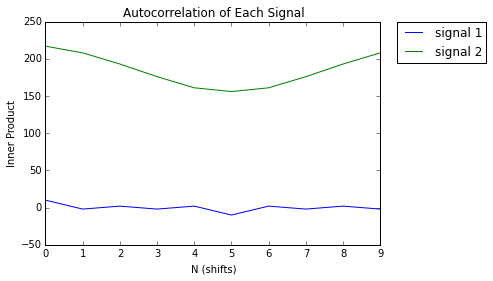
\includegraphics[scale=0.5]{autocorrelation.png}\end{center}
        \item \emph{cross-correlation}
        \begin{center}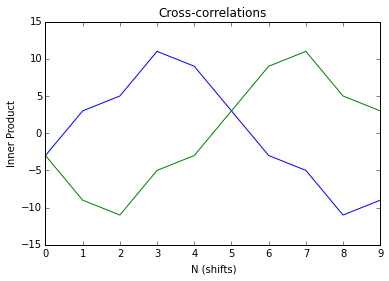
\includegraphics[scale=0.5]{cross-correlation.png}\end{center}
        
    \end{menumerate}
    
    \newpage
    \item \textbf{Inner products}
    \emph{Use the Cauchy-Schwarz inequality to verify (i.e. prove or derive) the triangle inequality:}
    \begin{equation*}
        \|\vec{x} + \vec{y}\| \leq \|\vec{x}\| + \|\vec{y}\|.
    \end{equation*}
    \begin{proof}
        Observe the following manipulation 
        \begin{equation*}
        \begin{aligned}
         \|x + y\|^2 &= \langle x + y, x+ y \rangle \\
            &=  \langle x, x \rangle + \langle x, y \rangle  + \langle y, x \rangle  + \langle y, y \rangle  \\
            &= \|x\|^2 + 2\langle x, y \rangle + \|y\|^2.
        \end{aligned}
        \end{equation*}
        Then by the Cauchy-Schwartz inequality we have that 
        \begin{equation*}
            \|x + y\|^2 \leq \|x\|^2 + 2\|x\|\|y\| + \|y\|^2 = (\|x\| + \|y\|)^2
        \end{equation*}
        Thus we have 
        \begin{equation*}
            \|x + y\| \leq \|x\| + \|y\|.
        \end{equation*}
    \end{proof}
    
    
    \newpage
    \item \textbf{Midterm Review}
    \\See attached scans
    
    \newpage
    \item \textbf{No more circuits :))!!!!} Replicate the projection equation from discussion in LaTeX without the ugly arrows on top like they do in textbooks, which would make Babak happy (not as easy as it sounds)\\
    \DeclarePairedDelimiter{\norm}{\lVert}{\rVert}
    \newcommand{\vectorproj}[2][]{\textit{proj}_{\vect{#1}}\vect{#2}}
    \newcommand{\vect}{\mathbf}
    \begin{equation*}
    \begin{aligned}
        \vectorproj[b]{a} &= \frac{\vect{a} \cdot \vect{b}}{\norm{\vect{b}}^2} \vect{b}\\
        &= \frac{\langle\vect{a}, \vect{b}\rangle}{\langle\vect{b}, \vect{b}\rangle} \vect{b}
    \end{aligned}
    \end{equation*}
    

\end{menumerate}

\end{document}
